\documentclass[letterpaper,oneside,12pt]{article}%twocolumn;titlepage(separate title page)
\usepackage{pslatex}                %Times New Roman Font; Improves on-screen readability; preferred to using times package
\usepackage[margin=0.5in]{geometry}   %1in 'uniform' margin (with oneside)
\usepackage{color}
\usepackage{amsmath}
\usepackage{amsfonts}
\usepackage{enumitem}
\usepackage{url}
\usepackage{bm}
\usepackage{graphicx}
\usepackage{optprog}
\usepackage{lscape}
\setcounter{MaxMatrixCols}{20}
%\setlength{\headsep}{0in}           %Distance from bottom of header to the body of text on a page.
\newcommand{\rem}[1]{}
\renewcommand{\arraystretch}{1}

% **********************************************************************
% Compact itemize, enumerate and description environments %pkg enumitem
% **********************************************************************
\usepackage{enumitem}            % [FAILS w/BEAMER] Lets define enumerate spacing: \begin{enumerate}[topsep=0pt,itemsep=0pt,parsep=0pt,partopsep=0pt]
\newenvironment{compitem}{\begin{itemize}[topsep=0pt,itemsep=0pt,parsep=0pt,partopsep=0pt]}{\end{itemize}}
\newenvironment{compenum}{\begin{enumerate}[topsep=0pt,itemsep=0pt,parsep=0pt,partopsep=0pt]}{\end{enumerate}}
\newenvironment{compdesc}{\begin{description}[topsep=0pt,itemsep=0pt,parsep=0pt,partopsep=0pt]}{\end{description}}

\DeclareMathOperator{\conv}{conv}
\DeclareMathOperator*{\proj}{proj}

\newcommand{\blu}{\color{blue}}
\newcommand{\bla}{\color{black}}
\begin{document}
\noindent\fbox{%
	\parbox{\textwidth}{%
		\begin{center}
		\textbf{\large{Department of Mathematics}} \\
		\textbf{\large{SA 405 - Advanced Mathematical Programming}} \\
		\textbf{\large{Quiz 7}}
		\end{center}
	}%
}

\vspace{3mm} \hspace{\fill} \textbf{Name: \underline{\hspace{6cm}}}

Suppose you are solving a maximization integer program via the branch and bound algorithm and at this iteration you have the following tree. Note that at this point, \textbf{you have just finished solving problem P5}. This means that you have not yet made any decisions based on the solution of problem P5!

\begin{center}
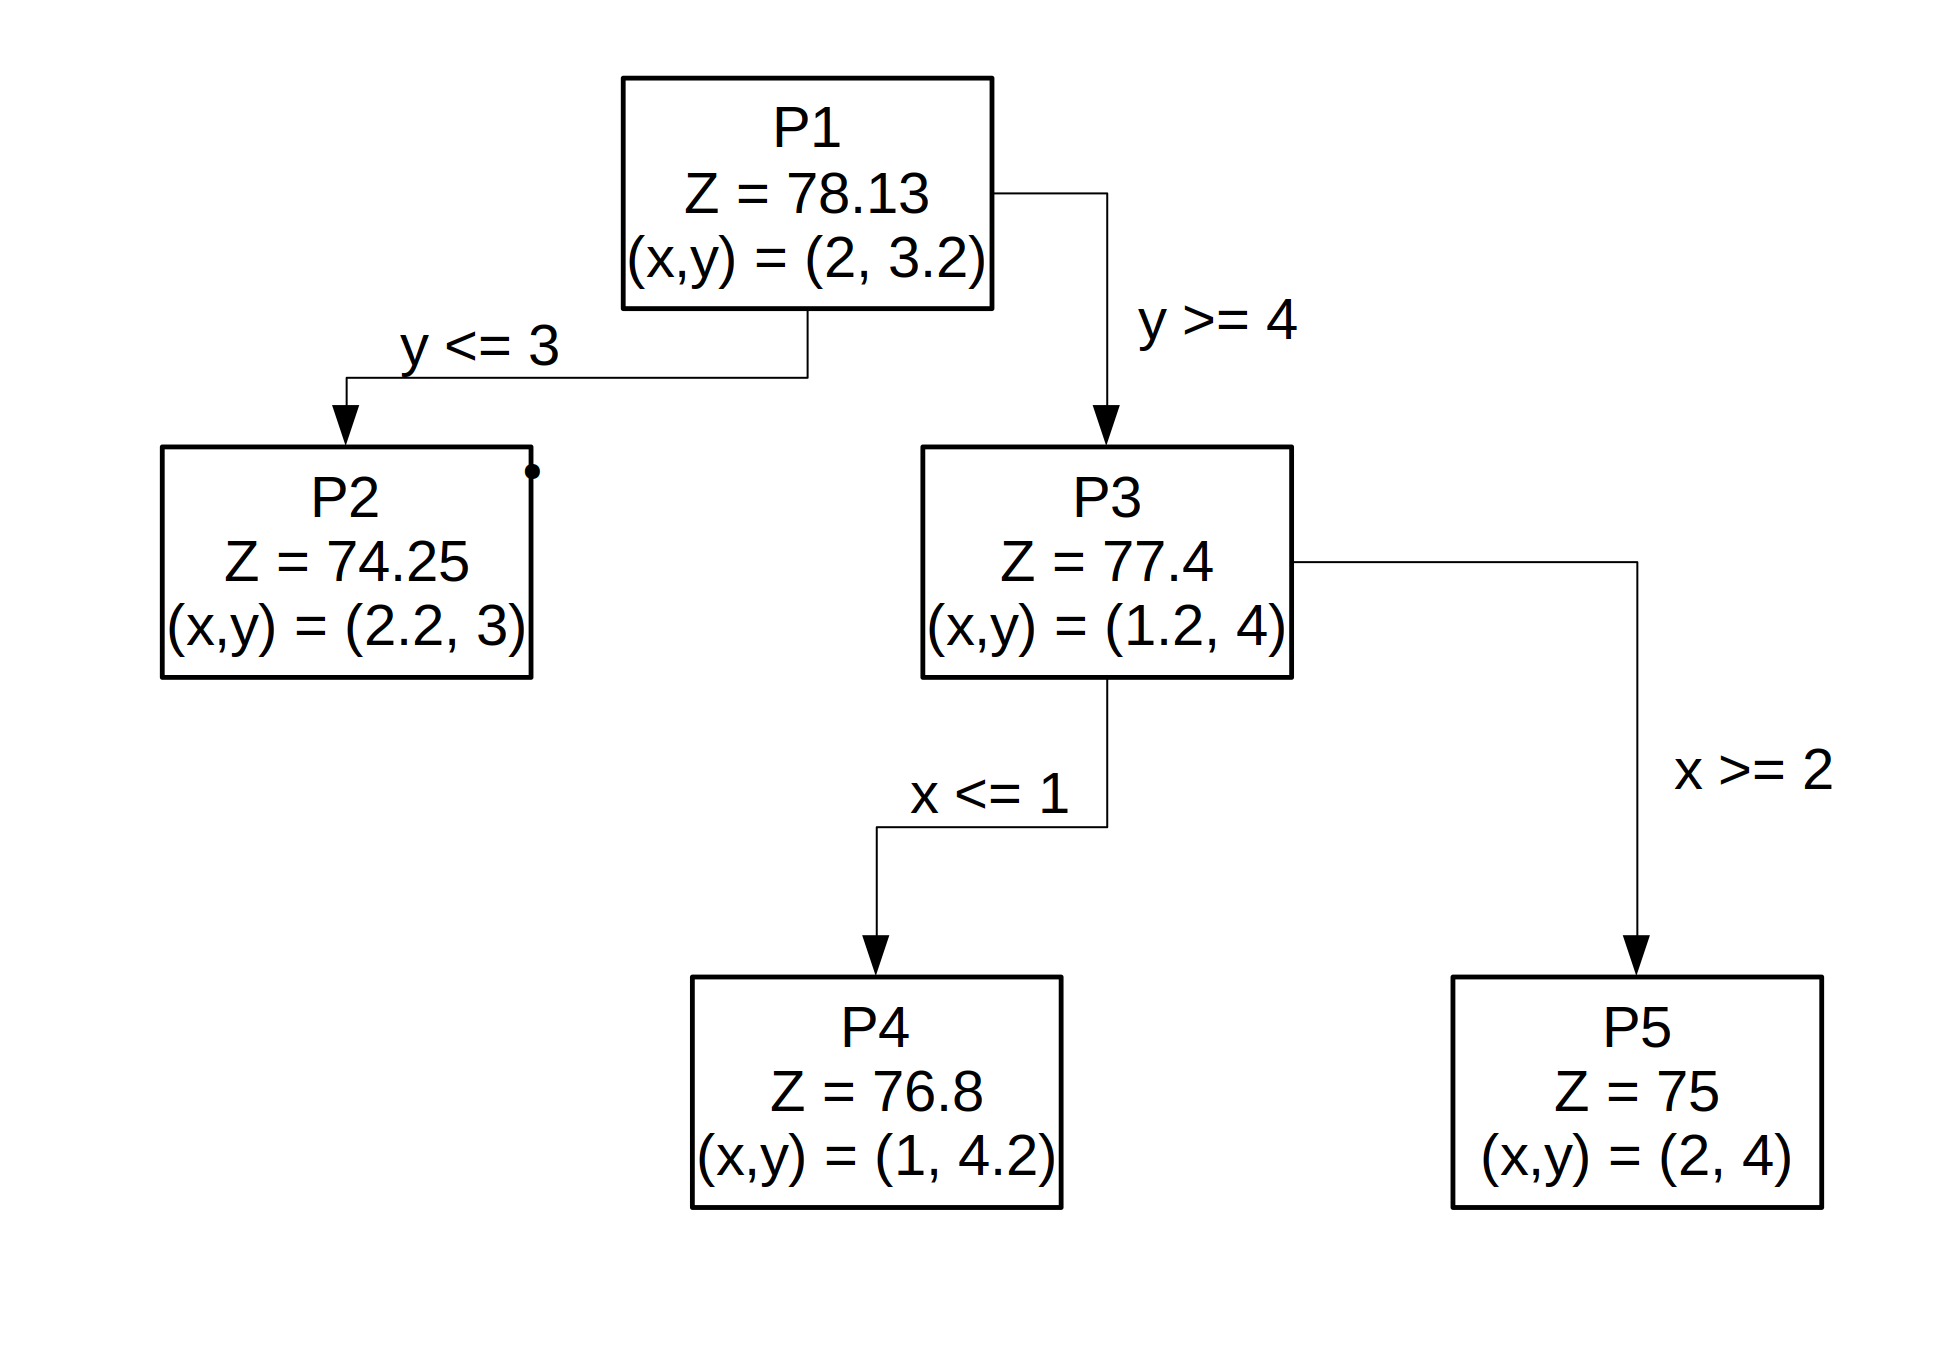
\includegraphics[width=0.60\textwidth]{B&B_example.png}
\end{center}

Answer the following questions.

\begin{enumerate}
\item (10 points) Which nodes in the tree are currently candidates for branching? \vfill
\item Let $z^*_{IP}$ denote the optimal objective function value of the integer program. 
	\begin{enumerate}
	\item (10 points) What is the current best upper bound on $z^*_{IP}$? \vfill
	\item (10 points) What is the current best lower bound on $z^*_{IP}$? \vfill
	\end{enumerate}	 
\newpage
\item (10 points) What is the current/incumbent solution in the tree? \vfill
	\begin{enumerate}
	\item (5 points) Is this current solution optimal? (YES \hspace{0.5cm} NO \hspace{0.5cm} DON'T KNOW YET). \vfill
	\item (5 points) If we allow a MIP gap of 5\% is this current solution optimal? (YES \hspace{0.5cm} NO) \vfill
	\end{enumerate}
\item (10 points) After solving problem P5, are there any nodes that can be eliminated from the tree? \vfill
\item Suppose we are using a strategy where we explore the region with the highest upper bound first.
	\begin{enumerate}
	\item (10 points) Which of the active nodes should we branch on? \vfill
	\item (15 points) What constraints would we add to this problem in order to generate our two new nodes (i.e., what variables are we branching on and what are the limits) \vfill
	\end{enumerate}
\item (15 points) Based on this tree, which of the following is \textbf{possible} for our final IP solution?
	\begin{enumerate}
	\item Unique optimal solution? (YES \hspace{0.5cm} NO)
	\item Multiple optimal solutions? (YES \hspace{0.5cm} NO)
	\item Infeasible? (YES \hspace{0.5cm} NO)
	\item Unbounded? (YES \hspace{0.5cm} NO)
	\item Our final solution is $x = (2,3.2)$ (YES \hspace{0.5cm} NO)
	\end{enumerate}
\end{enumerate}

\end{document}
